\chapter{纹理(Texturing)}
\begin{flushleft}
我们的演示渐渐变得有趣,真实世界的对象通常比每个对象的材料有更多的细节。 纹理映射是一种允许我们将图像数据映射到三角形上的技术,从而使我们能够显着增加场景的细节和真实感。 例如,我们可以通过在每一侧绘制板条纹理来构建一个立方体并将其转换为板条箱(图\ref{fig:9-1})。
\end{flushleft}

\begin{figure}[h]
    \label{fig:9-1}
    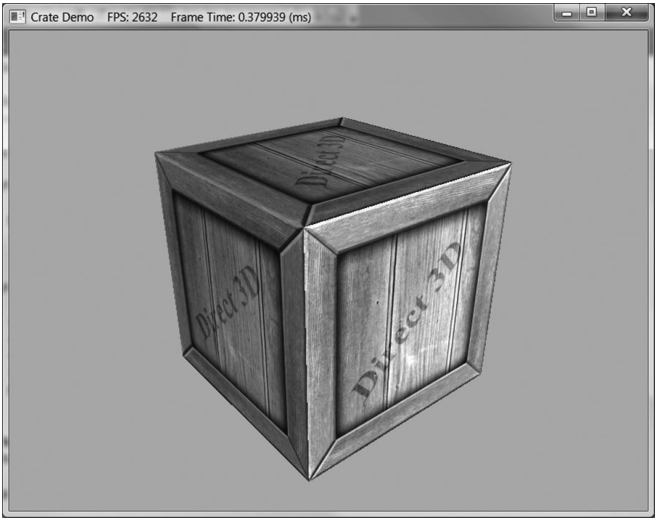
\includegraphics[width=\textwidth]{9-1}
    \centering
    \caption{Crate演示创建一个带有条板纹理的立方体。}
\end{figure}

\begin{flushleft}
当然,一般来说,模型越准确,计算成本越高; 因此,必须在现实主义和速度之间达成平衡。 例如,用于电影的3D特殊FX场景可以比游戏更复杂并且使用非常逼真的照明模型,因为电影的帧是预渲染的,因此它们可以花费数小时或数天来处理帧。 另一方面,游戏是实时应用程序,因此,帧需要以每秒至少30帧的速率绘制。\\
请注意,本书中解释和实现的照明模型很大程度上基于[Möller08]中描述的模型。\\
~\\
{\large Objectives:}
\begin{itemize}
    \item 1.了解如何指定映射到三角形的纹理部分。
    \item 2.了解如何创建并启用纹理。
    \item 3.了解如何过滤纹理以创建更平滑的图像。
    \item 4.了解如何使用地址模式多次平铺纹理。
    \item 5.了解如何组合多个纹理以创建新纹理和特殊效果。
    \item 6.学习如何通过纹理动画创建一些基本效果。
\end{itemize}
\end{flushleft}

%------- 9.1 ---------------
\section{纹理和资源回顾(Texture And Resource Recap)}
\begin{flushleft}
回想一下,自第4章以来我们已经使用了纹理; 深度缓冲区和后台缓冲区是由 ID3D12Resource 接口表示的2D纹理对象,D3D12\_RESOURCE\_DESC::Dimension 为 D3D12\_RESOURCE\_DIMENSION\_TEXTURE2D。为了便于参考,在第一部分中,我们将回顾第4章中已经介绍过的大部分纹理材料。\\

2D纹理是数据元素的矩阵。 2D纹理的一个用途是存储2D图像数据,其中纹理中的每个元素存储像素的颜色。 但是,这不是唯一的用法; 例如,在称为法线贴图的高级技术中,纹理中的每个元素都存储3D向量而不是颜色。 因此,尽管将纹理视为存储图像数据是常见的,但它们实际上更为通用。1D纹理(D3D12\_RESOURCE\_DIMENSION\_TEXTURE1D)类似于数据元素的1D阵列,3D纹理(D3D12\_RESOURCE\_DIMENSION\_TEXTURE3D)类似于数据元素的3D数组。 1D,2D和3D纹理界面均由通用ID3D12Resource表示。\\

纹理与缓冲区资源不同,缓冲区资源只存储数据数组; 纹理可以具有mipmap级别,GPU可以对它们执行特殊操作,例如应用过滤器和多重采样。 由于纹理资源支持这些特殊操作,它们仅限于某种数据格式,而缓冲资源可以存储任意数据。 纹理支持的数据格式由DXGI\_FORMAT枚举类型描述。 一些示例格式是:\\
\end{flushleft}

\begin{itemize}
  \item 1.DXGI\_FORMAT\_R32G32B32\_FLOAT:表示每个元素都是三个 32-bit的浮点型分量
  \item 2.DXGI\_FORMAT\_R16G16B16A16\_UNORM:每个元素都是四个 16-bit 的分量,取值范围在[0,1]
  \item 3.DXGI\_FORMAT\_R32G32\_UINT: 每个元素都是两个32-bit无符号整型分量
  \item 4.DXGI\_FORMAT\_R8G8B8A8\_UNORM: 每个元素都是四个 8-bit 无符号分量,取值范围在[0,1]
  \item 5.DXGI\_FORMAT\_R8G8B8A8\_SNORM: 每个元素都是四个 8-bit 有符号分量,取值范围在[-1, 1]
  \item 6.DXGI\_FORMAT\_R8G8B8A8\_SINT: 每个元素都是四个 8-bit 有符号整型分量,取值范围在[-128,127]
  \item 7.DXGI\_FORMAT\_R8G8B8A8\_UINT: 每个元素都是四个 8-bit 无符号整型分量,取值范围在[0, 255]
  \item 8.DXGI\_FORMAT\_R16G16B16A16\_TYPELESS: 每个元素都是四个 16-bit 的分量,可以在后面处理过程中,重新解释为其他类型 注:R、G、B、A分别表示red, green, blue, alpha
\end{itemize}

\begin{flushleft}
请注意,R、G、B、A字母分别代表红色、绿色、蓝色和透明度。 正如我们之前所说,纹理不需要存储颜色信息;举个例子,格式 DXGI\_FORMAT\_R32G32B32\_FLOAT 有三个浮点型分量,可以存储具有浮点坐标的3D矢量(不一定是颜色矢量)。 还有无类型格式,只保留内存,然后指定当纹理绑定到渲染管道时如何在以后重新解释数据(有点像转换); 例如,以下无类型格式保留具有四个8位分量的元素,但不指定数据类型(例如,整数,浮点,无符号整数):DXGI\_FORMAT\_R16G16B16A16\_TYPELESS。\\
~\\
NOTICE: DirectX 11 SDK文档说:“创建完全类型的资源会使资源限制为使用它创建的格式。 这使运行时能够优化访问[...]。“因此,如果您真的需要,您应该只创建无类型资源; 否则,创建一个完全类型的资源。\\
~\\
纹理可以绑定到渲染管道的不同阶段;一个常见的例子是使用纹理作为渲染目标(即Direct3D绘制到纹理中)和作为着色器资源(即,纹理将在着色器中采样)。纹理既可以用作渲染目标,也可以用作着色器资源,但不能同时使用。渲染到纹理然后将其用作着色器资源,一种称为渲染到纹理的方法允许一些有趣的特殊效果,我们将在本书后面使用它们。对于要用作渲染目标和着色器资源的纹理,我们需要为该纹理资源创建两个描述符:(1)一个存在于渲染目标堆中(即D3D12\_DESCRIPTOR\_HEAP\_TYPE\_RTV)和(2)存在于其中的一个着色器资源堆(即D3D12\_DESCRIPTOR\_HEAP\_TYPE\_CBV\_SRV\_UAV)。 (请注意,着色器资源堆还可以存储常量缓冲区视图描述符和无序访问视图描述符。)然后,资源可以绑定为渲染目标,或绑定为根签名中的根参数的着色器输入(但从不在同时):\\
\end{flushleft}

\begin{lstlisting}
// Bind as render target.
CD3DX12_CPU_DESCRIPTOR_HANDLE rtv = ...;
CD3DX12_CPU_DESCRIPTOR_HANDLE dsv = ...;
cmdList->OMSetRenderTargets(1, &rtv, true, &dsv);
// Bind as shader input to root parameter.
CD3DX12_GPU_DESCRIPTOR_HANDLE tex = ...;
cmdList->SetGraphicsRootDescriptorTable(rootParamIndex, tex);
\end{lstlisting}

\begin{flushleft}
资源描述符基本上做了两件事:它们告诉Direct3D资源将如何使用(即,您将绑定它的管道的哪个阶段),如果资源格式在创建时被指定为无类型,那么现在必须在创建视图时声明类型。 因此,对于无类型格式,纹理的元素可以在一个管道阶段中被视为浮点值,而在另一个管道阶段中被视为整数; 这基本上相当于对数据的重新解释。\\
在本章中,我们只对将纹理绑定为着色器资源感兴趣,以便我们的像素着色器可以对纹理进行采样来着色像素。\\
\end{flushleft}

%------- 9.2 ---------------
\section{纹理坐标(Texture Coordinates)}
\begin{flushleft}
Direct3D使用纹理坐标系,该坐标系包含一个水平延伸到图像的$u$轴和一个垂直于图像运行的$v$轴。 坐标$(u,v)$使得$0\leq u,v\leq 1$,将纹理上的元素称为纹素(texel)。 请注意,$v$轴在“向下”方向上为正(参见图\ref{fig:9-2})。另外,请注意使用的归一化坐标间隔$[0,1]$,因为它为Direct3D提供了与维度无关的范围; 例如,无论实际纹理尺寸是$256\times 256$,$512\times 1024$还是$2048\times 2048$像素,$(0.5,0.5)$总是指定中间纹理像素。 同样地,$(0.25,0.75)$将纹理元素识别为水平方向上总宽度的四分之一,以及垂直方向上总高度的四分之三。 目前,纹理坐标始终在$[0,1]$范围内,但稍后我们将解释当您超出此范围时会发生什么。
\end{flushleft}

\begin{figure}[h]
    \label{fig:9-2}
    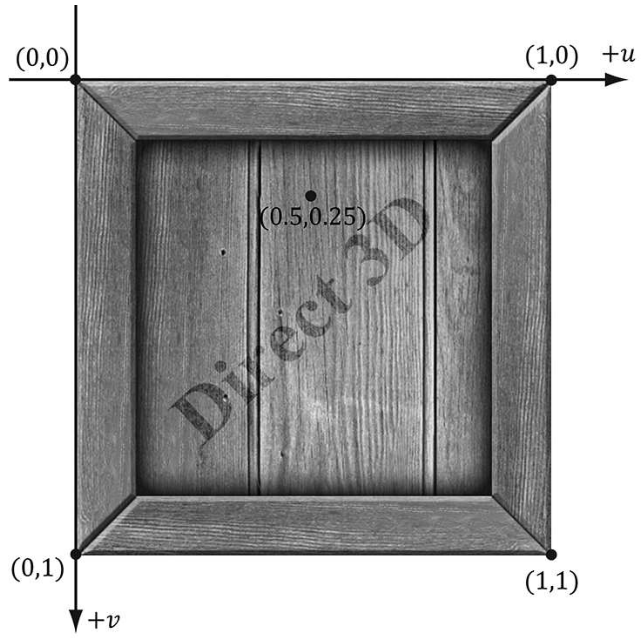
\includegraphics[width=\textwidth]{9-2}
    \centering
    \caption{纹理坐标系,有时称为纹理空间。}
\end{figure}

\begin{figure}[h]
    \label{fig:9-3}
    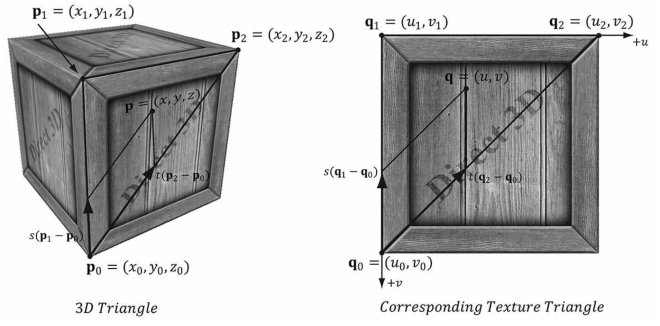
\includegraphics[width=\textwidth]{9-3}
    \centering
    \caption{左边是三维空间中的三角形,右边是我们在纹理上定义一个2D三角形,它将被映射到3D三角形上。}
\end{figure}

\begin{flushleft}
对于每个3D三角形,要在纹理上定义一个相应的三角形,以映射到3D三角形上(参见图\ref{fig:9-3})。 令$p_{0}$,$p_{1}$和$p_{2}$为具有相应纹理坐标$q_{0}$,$q_{1}$和$q_{2}$的3D三角形的顶点。 对于3D三角形上的任意点$(x,y,z)$,通过使用相同的$s$,$t$参数对3D三角形上的顶点纹理坐标进行线性插值来找到其纹理坐标$(u,v)$;即\\
如果 \\
\end{flushleft}
\begin{align*}
(x,y,z)=p=p_{0}+s(p_{1}-p_{0})+t(p_{2}-p_{0})\\
\end{align*}
\begin{flushleft}
对于 $s\geq 0,t\geq 0,s+t\leq 1$ 则,\\
\end{flushleft}
\begin{align*}
(u,v)=q=q_{0}+s(q_{1}-q_{0})+t(q_{2}-q_{0})
\end{align*}
\begin{flushleft}
这样,三角形上的每个点都有一个相应的纹理坐标。\\
为了实现这一点,需要再次修改顶点结构,并添加一对纹理坐标,用于标识纹理上的一个点。 现在每个3D顶点都有一个相应的2D纹理顶点。 因此,由三个顶点定义的每个3D三角形也在纹理空间中定义2D三角形(即,我们已经为每个3D三角形关联了2D纹理三角形)。\\
\end{flushleft}

\begin{lstlisting}
struct Vertex
{
    DirectX::XMFLOAT3 Pos;
    DirectX::XMFLOAT3 Normal;
    DirectX::XMFLOAT2 TexC;
};

std::vector<D3D12_INPUT_ELEMENT_DESC> mInputLayout =
{
    { "POSITION", 0, DXGI_FORMAT_R32G32B32_FLOAT, 0, 0,
       D3D12_INPUT_CLASSIFICATION_PER_VERTEX_DATA, 0 },
    { "NORMAL", 0, DXGI_FORMAT_R32G32B32_FLOAT, 0, 12,
       D3D12_INPUT_CLASSIFICATION_PER_VERTEX_DATA, 0 },
    { "TEXCOORD", 0, DXGI_FORMAT_R32G32_FLOAT, 0, 24,
       D3D12_INPUT_CLASSIFICATION_PER_VERTEX_DATA, 0 },
};
\end{lstlisting}

\begin{flushleft}
~\\
NOTICE: 您可以创建“奇数”纹理映射,其中2D纹理三角形与3D三角形有很大不同。 因此,当2D纹理被映射到3D三角形时,发生大量拉伸和扭曲,使得结果看起来不好。 例如,将锐角三角形映射到直角三角形需要拉伸。 通常,纹理失真应该最小化,除非纹理艺术家需要失真外观。\\
~\\
请注意,在图\ref{fig:9-3}中,我们将整个纹理图像映射到立方体的每个面上。这绝不是必需的。 可以将纹理的子集映射到几何体上。 实际上,我们可以在一个大的纹理贴图上放置几个不相关的图像(这称为纹理图集),并将其用于几个不同的对象(图\ref{fig:9-4})。 纹理坐标将决定纹理的哪个部分映射到三角形。\\
\end{flushleft}

\begin{figure}[h]
    \label{fig:9-4}
    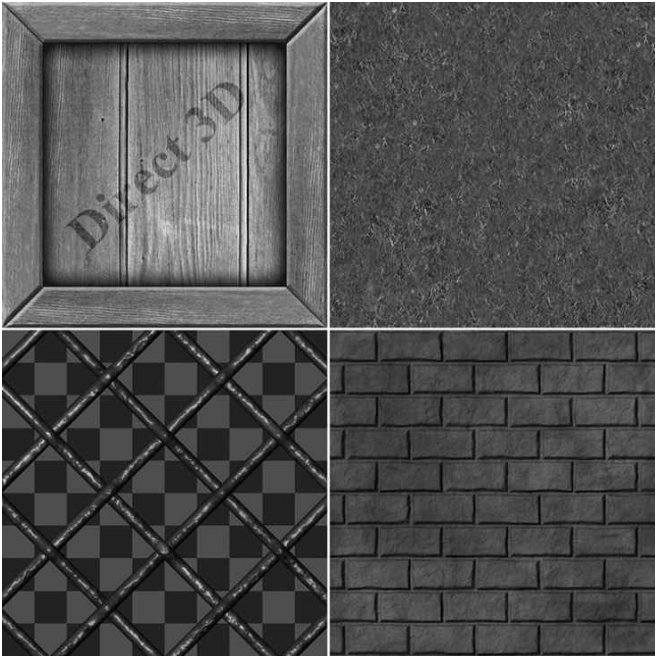
\includegraphics[width=\textwidth]{9-4}
    \centering
    \caption{在一个大纹理上存储四个子纹理的纹理图集。 设置每个顶点的纹理坐标,以便将纹理的所需部分映射到几何体上。}
\end{figure}

%------- 9.3 ---------------
\section{纹理数据源(Texture Data Sources)}
\begin{flushleft}
为游戏创建纹理的最流行的方法是让艺术家在Photoshop或其他图像编辑器中制作它们,然后将它们保存为图像文件,如BMP,DDS,TGA或PNG。 然后游戏应用程序将加载时的图像数据加载到ID3D12Resource对象中。 对于实时图形应用程序,DDS(DirectDraw表面格式)图像文件格式是首选,因为它支持GPU本身理解的各种图像格式; 特别是,它支持可由GPU本机解压缩的压缩图像格式。\\
~\\
NOTICE: 艺术家不应将DDS格式用作工作图像格式。相反,他们应该使用他们喜欢的格式来保存工作。 然后,当纹理完成时,它们会导出到DDS以用于游戏应用程序。
~\\
\end{flushleft}

%------- 9.3.1 ---------------
\subsection{DDS 概览(DDS Overview)}
\begin{flushleft}
DDS格式是3D图形的理想选择,因为它支持专门用于3D图形的特殊格式和纹理类型。 它本质上是为GPU构建的图像格式。例如,DDS纹理支持3D图形开发中使用的以下功能(尚未讨论):\\
\end{flushleft}

\begin{itemize} 
  \item 1.贴图(mipmaps)
  \item 2.GPU可以本地解压缩的压缩格式
  \item 3.纹理数组
  \item 4.立方体贴图
  \item 5.体积纹理
\end{itemize}

\begin{flushleft}
DDS格式可以支持不同的像素格式。 像素格式由DXGI\_FORMAT枚举类型的成员描述; 但是,并非所有格式都适用于DDS纹理。通常,对于未压缩的图像数据,您将使用以下格式:\\
\end{flushleft}

\begin{itemize} 
  \item 1.DXGI\_FORMAT\_B8G8R8A8\_UNORM 或 DXGI\_FORMAT\_B8G8R8X8\_UNORM:用于低动态范围的图像。
  \item 2.DXGI\_FORMAT\_R16G16B16A16\_FLOAT:用于高动态范围图像。
\end{itemize}

\begin{flushleft}
随着虚拟世界随着数百个纹理的增长,纹理的GPU内存需求迅速增加(请记住,我们需要将所有这些纹理保留在GPU内存中以便快速应用它们)。 为了帮助减轻这些内存需求,Direct3D支持压缩纹理格式:BC1,BC2,BC3,BC4,BC5,BC6和BC7:\\
\end{flushleft}

\begin{itemize} 
  \item 1.BC1(DXGI\_FORMAT\_BC1\_UNORM):如果需要压缩支持三种颜色通道的格式,并且只需要一个1位(开/关)alpha分量,请使用此格式。
  \item 2.BC2(DXGI\_FORMAT\_BC2\_UNORM):如果需要压缩支持三种颜色通道的格式,并且只需要一个4位alpha分量,请使用此格式。
  \item 3.BC3(DXGI\_FORMAT\_BC3\_UNORM):如果需要压缩支持三种颜色通道的格式和8位alpha分量,请使用此格式。
  \item 4.BC4(DXGI\_FORMAT\_BC4\_UNORM):如果需要压缩包含一个颜色通道的格式(例如,灰度图像),请使用此格式。
  \item 5.BC5(DXGI\_FORMAT\_BC5\_UNORM):如果需要压缩支持两种颜色通道的格式,请使用此格式。
  \item 6.BC6(DXGI\_FORMAT\_BC6\_UF16):将此格式用于压缩HDR(高动态范围)图像数据。
  \item 7.BC7(DXGI\_FORMAT\_BC7\_UNORM):使用此格式进行高质量RGBA压缩。 这种格式显着减少了压缩法线贴图造成的错误。
\end{itemize}

\begin{flushleft}
~\\
NOTICE: 压缩纹理只能用作渲染管道的着色器阶段的输入,而不能用作渲染目标。\\
NOTICE: 因为块压缩算法适用于$4\times 4$像素块,所以纹理的尺寸必须是4的倍数。\\
~\\
同样,这些格式的优点是它们可以压缩存储在GPU内存中,然后在需要时由GPU即时解压缩。 存储压缩在DDS文件中的纹理的另一个好处是它们也占用较少的硬盘空间。
\end{flushleft}

%------- 9.3.2 ---------------
\subsection{创建 DDS 文件(Createing DDS Files)}
\begin{flushleft}
如果您不熟悉图形编程,您可能不熟悉DDS,可能更习惯使用BMP,TGA或PNG等格式。 以下是将传统图像格式转换为DDS格式的两种方法:\\
\end{flushleft}

\begin{itemize} 
  \item 1.NVIDIA为Adobe Photoshop提供了一个插件,可以将图像导出为DDS格式。 该插件可在https://developer.nvidia.com/nvidia-texture-tools-adobe-photoshop 获得。 在其他选项中,它允许您指定DDS文件的DXGI\_FORMAT,并生成贴图。
  \item 2.Microsoft提供了一个名为texconv的命令行工具,可用于将传统图像格式转换为DDS。 此外,texconv程序还有其他功能,例如调整图像大小,更改像素格式,生成mipmap及其他。 您可以在以下网站https://directxtex.codeplex.com/wikipage?title=Texconv\&referringTitle=Documentation找到文档和下载链接。
\end{itemize}

\begin{flushleft}
以下示例输入BMP文件 bricks.bmp 以格式 BC3\_UNORM 输出DDS文件 bricks.dds 生成具有10个mipmap的mipmap链。
\end{flushleft}

\begin{lstlisting}
texconv -m 10 -f BC3_UNORM treeArray.dds
\end{lstlisting}

\begin{flushleft}
~\\
NOTICE:  Microsoft提供了一个名为texassemble的附加命令行工具,用于创建存储纹理数组,体积贴图和立方体贴图的DDS文件。 我们将在本书的后面部分使用此工具。其文档和下载链接可以在https://directxtex.codeplex.com/wikipage?title=Texassemble\&referringTitle=Documentation 找到。\\
~\\
NOTICE: Visual Studio 2015具有内置的图像编辑器,除了其他流行的格式外,还支持DDS。 您可以将图像拖到Visual Studio 2015中,它应该在图像编辑器中打开它。 对于DDS文件,您可以查看mipmap级别,更改DDS格式以及查看各种颜色通道。\\
\end{flushleft}

%------- 9.4---------------
\section{创建并启用纹理(Creating and Enabling a Texture)}

%------- 9.4.1 ---------------
\subsection{加载(Loading DDS Files)}
\begin{flushleft}
Microsoft提供了简单的加载 DDS 文件的源码,见 https://github.com/Microsoft/DirectXTK/wiki/DDSTextureLoader 。\\
然而,在撰写本文时,代码仅支持DirectX 11.我们修改了DDSTextureLoader.h / .cpp文件并为DirectX 12提供了另一种方法(这些修改过的文件可以在DVD上的Common文件夹中或者可下载的来源中找到):\\
\end{flushleft}

\begin{lstlisting}
HRESULT DirectX::CreateDDSTextureFromFile12(
    _In_ ID3D12Device* device,
    _In_ ID3D12GraphicsCommandList* cmdList,
    _In_z_ const wchar_t* szFileName,
    _Out_ Microsoft::WRL::ComPtr<ID3D12Resource>& texture,
    _Out_ Microsoft::WRL::ComPtr<ID3D12Resource>& textureUploadHeap);
\end{lstlisting}

\begin{itemize}
  \item 1.device: 指向D3D设备创建纹理资源的指针。
  \item 2.cmdList: 用于提交GPU命令的命令列表(例如,将纹理数据从上载堆复制到默认堆)。
  \item 3.szFileName: 要加载的图像的文件名。
  \item 4.texture: 使用加载的图像数据返回纹理资源。
  \item 5.textureUploadHeap: 返回用作上传堆(Upload Heap)的纹理资源,用来将图像数据复制到默认堆纹理资源中。 在GPU完成复制命令之前,不能销毁此资源。
\end{itemize}

\begin{flushleft}
要从名为WoodCreate01.dds的图像创建纹理,我们将编写以下内容:\\
\end{flushleft}

\begin{lstlisting}
struct Texture
{
    // Unique material name for lookup.
    std::string Name;
    std::wstring Filename;
    Microsoft::WRL::ComPtr<ID3D12Resource> Resource = nullptr;
    Microsoft::WRL::ComPtr<ID3D12Resource> UploadHeap = nullptr;
};

auto woodCrateTex = std::make_unique<Texture>();
woodCrateTex->Name = "woodCrateTex";
woodCrateTex->Filename = L”Textures/WoodCrate01.dds”;
ThrowIfFailed(DirectX::CreateDDSTextureFromFile12(
    md3dDevice.Get(), mCommandList.Get(),
    woodCrateTex->Filename.c_str(),
    woodCrateTex->Resource, 
    woodCrateTex->UploadHeap));
\end{lstlisting}

%------- 9.4.2 ---------------
\subsection{SRV 堆(SRV Heap)}
\begin{flushleft}
一旦创建了纹理资源,我们需要为它创建一个SRV描述符,我们可以将其设置为根签名参数槽以供着色器程序使用。 为此,我们首先需要使用 ID3D12Device::CreateDescriptorHeap 创建描述符堆来存储SRV描述符。 以下代码构建一个具有三个描述符的堆,这些描述符可以存储CBV,SRV或UAV描述符,并且对着色器可见:\\
\end{flushleft}

\begin{lstlisting}
D3D12_DESCRIPTOR_HEAP_DESC srvHeapDesc = {};
srvHeapDesc.NumDescriptors = 3;
srvHeapDesc.Type = D3D12_DESCRIPTOR_HEAP_TYPE_CBV_SRV_UAV;
srvHeapDesc.Flags = D3D12_DESCRIPTOR_HEAP_FLAG_SHADER_VISIBLE;
ThrowIfFailed(md3dDevice->CreateDescriptorHeap(
    &srvHeapDesc, IID_PPV_ARGS(&mSrvDescriptorHeap)));
\end{lstlisting}

%------- 9.4.3 ---------------
\subsection{创建 SRV 描述符(Creating SRV Descriptors)}
\begin{flushleft}
一旦我们有了SRV堆,我们就需要创建实际的描述符。 通过填写 D3D12\_SHADER\_RESOURCE\_VIEW\_DESC 对象来描述SRV描述符,该对象描述资源的使用方式和其他信息——其格式、维度、mipmaps计数等。\\
\end{flushleft}

\begin{lstlisting}
typedef struct D3D12_SHADER_RESOURCE_VIEW_DESC
{
    DXGI_FORMAT Format;
    D3D12_SRV_DIMENSION ViewDimension;
    UINT Shader4ComponentMapping;
    union
    {
        D3D12_BUFFER_SRV Buffer;
        D3D12_TEX1D_SRV Texture1D;
        D3D12_TEX1D_ARRAY_SRV Texture1DArray;
        D3D12_TEX2D_SRV Texture2D;
        D3D12_TEX2D_ARRAY_SRV Texture2DArray;
        D3D12_TEX2DMS_SRV Texture2DMS;
        D3D12_TEX2DMS_ARRAY_SRV Texture2DMSArray;
        D3D12_TEX3D_SRV Texture3D;
        D3D12_TEXCUBE_SRV TextureCube;
        D3D12_TEXCUBE_ARRAY_SRV TextureCubeArray;
    };
} D3D12_SHADER_RESOURCE_VIEW_DESC;

typedef struct D3D12_TEX2D_SRV
{
    UINT MostDetailedMip;
    UINT MipLevels;
    UINT PlaneSlice;
    FLOAT ResourceMinLODClamp;
} D3D12_TEX2D_SRV;
\end{lstlisting}

\begin{flushleft}
对于2D纹理,我们只关注 union 的 D3D12\_TEX2D\_SRV 部分。\\
\end{flushleft}

\begin{flushleft}
1.Format: 资源的格式。 如果格式为非无类型,则在创建视图时设置该值的DXGI\_FORMAT。 如果在创建期间为资源指定了无类型DXGI\_FORMAT,则必须在此处为视图指定非无类型格式,以便GPU知道如何解释数据。\\

2.ViewDimension: 资源维度; 目前,我们正在使用2D纹理,因此我们指定D3D12\_SRV\_DIMENSION\_TEXTURE2D。 其他常见的纹理尺寸为:\\
\end{flushleft}

\begin{itemize}
  \item 1.D3D12\_SRV\_DIMENSION\_TEXTURE1D: 1D 纹理资源
  \item 2.D3D12\_SRV\_DIMENSION\_TEXTURE3D: 3D 纹理资源
  \item 3.D3D12\_SRV\_DIMENSION\_TEXTURECUBE: 立方体纹理资源。
\end{itemize}

\begin{flushleft}
3.Shader4ComponentMapping: 在着色器中对纹理进行采样时,它将返回指定纹理坐标处的纹理数据的向量。 此字段提供了一种当重新排序采样纹理时返回向量分量的方法。 例如,您可以使用此字段交换红色和绿色分量。这将用于特殊情况,我们在本书中不需要这些情况。 所以我们只指定 D3D12\_DEFAULT\_SHADER\_4\_COMPONENT\_MAPPING,它不会对分量重新排序,只是按照它存储在纹理资源中的顺序返回数据。\\

4.MostDetailedMip: 指定要查看的最详细的mipmap级别的索引。这将是介于 $0$ 和 $MipCount-1$ 之间的数字。\\

5.MipLevels: 要查看的mipmap级别数,从MostDetailedMip开始。 此字段与MostDetailedMip一起允许我们指定要查看的mipmap级别的子范围。您可以指定$-1$以指示查看从MostDetailedMip到最后一个mipmap级别的所有mipmap级别。\\

6.PlaneSlice: 平面索引。\\

7.ResourceMinLODClamp: 指定可以访问的最小mipmap级别。0.0表示可以访问所有mipmap级别。 指定3.0表示可以访问mipmap级别3.0到$MipCount-1$。\\

下面用三个资源的实际描述符填充上一节中创建的堆:\\
\end{flushleft}

\begin{lstlisting}
// Suppose the following texture resources are already created.
// ID3D12Resource* bricksTex;
// ID3D12Resource* stoneTex;
// ID3D12Resource* tileTex;
// Get pointer to the start of the heap.
CD3DX12_CPU_DESCRIPTOR_HANDLE hDescriptor(
    mSrvDescriptorHeap->GetCPUDescriptorHandleForHeapStart());
D3D12_SHADER_RESOURCE_VIEW_DESC srvDesc = {};
srvDesc.Shader4ComponentMapping = 
    D3D12_DEFAULT_SHADER_4_COMPONENT_MAPPING;
srvDesc.Format = bricksTex->GetDesc().Format;
srvDesc.ViewDimension = D3D12_SRV_DIMENSION_TEXTURE2D;
srvDesc.Texture2D.MostDetailedMip = 0;
srvDesc.Texture2D.MipLevels = bricksTex->GetDesc().MipLevels;
srvDesc.Texture2D.ResourceMinLODClamp = 0.0f;
md3dDevice->CreateShaderResourceView(
    bricksTex.Get(),
    &srvDesc, hDescriptor);
// offset to next descriptor in heap
hDescriptor.Offset(1, mCbvSrvDescriptorSize);
srvDesc.Format = stoneTex->GetDesc().Format;
srvDesc.Texture2D.MipLevels = 
    stoneTex->GetDesc().MipLevels;
md3dDevice->CreateShaderResourceView(
    stoneTex.Get(),
    &srvDesc, hDescriptor);
// offset to next descriptor in heap
hDescriptor.Offset(1, mCbvSrvDescriptorSize);
srvDesc.Format = tileTex->GetDesc().Format;
srvDesc.Texture2D.MipLevels = 
    tileTex->GetDesc().MipLevels;
md3dDevice->CreateShaderResourceView(
    tileTex.Get(),
    &srvDesc, hDescriptor);
\end{lstlisting}

%------- 9.4.4 ---------------
\subsection{绑定纹理到管道中(Binding Textures to the Pipeline)}
\begin{flushleft}
现在通过更改材料常量缓冲区来指定每个绘制调用的材质。 这意味着绘制调用中的所有几何体都将具有相同的材质值。 这样产生的效果很局限,因为无法指定每个像素的材质变化,所以场景缺乏细节。 使用纹理贴图替代材质常量缓冲区能允许每个像素的变化,提高场景的细节和真实感,如图\ref{fig:9-1}所示。\\

在本章中,添加一个漫反射反照率纹理贴图来指定材质的漫反射反照率分量。 FresnelR0 和 Roughness 材质值仍将通过材质常数缓冲区以每个绘制调用频率指定; 但是,在“法线贴图”一章中,我们将介绍如何使用纹理来指定每像素级别的粗糙度。 请注意,通过纹理化,我们仍然会将 DiffuseAlbedo 组件保留在材质常量缓冲区中。 实际上,将在像素着色器中以下列方式将其与纹理漫反射反照率值组合:\\
\end{flushleft}

\begin{lstlisting}
// Get diffuse albedo at this pixel from texture.
float4 texDiffuseAlbedo = gDiffuseMap.Sample(
    gsamAnisotropicWrap, pin.TexC);
// Multiple texture sample with constant buffer albedo.
float4 diffuseAlbedo = texDiffuseAlbedo * gDiffuseAlbedo;
\end{lstlisting}

\begin{flushleft}
通常,我们将设置 DiffuseAlbedo=(1,1,1,1),这样就能不修改 texDiffuseAlbedo。 但是,有时稍微调整漫反射反照率而不创建新纹理是有效的。 例如,假设我们有一个砖纹理,而艺术家想要略微淡化蓝色。 这可以通过设置 DiffuseAlbedo=(0.9,0.9,1,1) 来减少红色和绿色成分来实现。\\

在材质定义中添加一个索引(该索引引用描述符堆中的SRV),指定与材质关联的纹理:\\
\end{flushleft}

\begin{lstlisting}
struct Material
{
    ...
    // Index into SRV heap for diffuse texture
    int DiffuseSrvHeapIndex = -1;
    ...
}
\end{lstlisting}

\begin{flushleft}
然后,假设已经定义了根签名以期望将着色器资源视图表绑定到第0个槽参数,我们可以使用以下代码绘制具有纹理的渲染项:\\
\end{flushleft}

\begin{lstlisting}
void CrateApp::DrawRenderItems(
ID3D12GraphicsCommandList* cmdList,
const std::vector<RenderItem*>& ritems)
{
    UINT objCBByteSize =
        d3dUtil::CalcConstantBufferByteSize(
            sizeof(ObjectConstants));
    UINT matCBByteSize =
        d3dUtil::CalcConstantBufferByteSize(
            sizeof(MaterialConstants));
    auto objectCB = mCurrFrameResource->
        ObjectCB->Resource();
    auto matCB = mCurrFrameResource->
        MaterialCB->Resource();
    // For each render item…
    for(size_t i = 0; i < ritems.size(); ++i)
    {
        auto ri = ritems[i];
        cmdList->IASetVertexBuffers(0, 1, 
            &ri->Geo->VertexBufferView());
        cmdList->IASetIndexBuffer(
            &ri->Geo->IndexBufferView());
        cmdList->IASetPrimitiveTopology(
            ri->PrimitiveType);
        CD3DX12_GPU_DESCRIPTOR_HANDLE tex(
            mSrvDescriptorHeap->
                GetGPUDescriptorHandleForHeapStart());
        tex.Offset(ri->Mat->DiffuseSrvHeapIndex, 
            mCbvSrvDescriptorSize);
        D3D12_GPU_VIRTUAL_ADDRESS objCBAddress =
            objectCB->GetGPUVirtualAddress() +
            ri->ObjCBIndex*objCBByteSize;
        D3D12_GPU_VIRTUAL_ADDRESS matCBAddress =
            matCB->GetGPUVirtualAddress() +
            ri->Mat->MatCBIndex*matCBByteSize;
        cmdList->SetGraphicsRootDescriptorTable(0, tex);
        cmdList->SetGraphicsRootConstantBufferView(1,
            objCBAddress);
        cmdList->SetGraphicsRootConstantBufferView(3,
            matCBAddress);
        cmdList->DrawIndexedInstanced(
            ri->IndexCount,
            1, 
            ri->StartIndexLocation,
            ri->BaseVertexLocation, 
            0);
    }
}
\end{lstlisting}

\begin{flushleft}
~\\
NOTICE: 任何着色器(顶点,几何或像素着色器)实际上都可以使用纹理资源。 现在,我们将在像素着色器中使用它们。 正如我们所提到的,纹理本质上是支持GPU上特殊操作的特殊数组,所以不难想象它们在其他着色器程序中也很有用。\\
~\\

NOTICE: 纹理图集可以提高性能,因为它可以通过一次绘制调用绘制更多几何图形。 例如,假设我们使用了如图\ref{fig:9-4}所示的纹理图集,其中包含板条箱,草和砖纹理。 然后,通过将每个对象的纹理坐标调整到其对应的子纹理,我们可以将所有几何体放在一个渲染项中(假设每个对象不需要更改其他参数)。 绘制调用有开销,因此最好使用这样的技术将开销降到最低,尽管我们注意到与早期版本的Direct3D相比,Direct3D 12的开销显著降低。\\
~\\
\end{flushleft}

%------- 9.5 ---------------
\section{滤镜(Filters)}
%------- 9.5.1 ---------------
\subsection{放大(Magnification)}
\begin{flushleft}
纹理贴图的元素应该被认为是来自连续图像的离散颜色样本;它们不应该被认为是带有区域的矩形。所以问题是:如果我们的纹理坐标$(u,v)$与其中一个纹素点不一致,会发生什么?这可能发生在以下情况中。假设玩家放大场景中的墙壁,使墙壁覆盖整个屏幕。例如,假设显示器分辨率为$1024\times 1024$,墙壁的纹理分辨率为$256\times 256$。需要进行纹理放大——试图用几个纹素覆盖许多像素。在例子中,每个texel点之间有四个像素。当顶点纹理坐标在三角形上插值时,每个像素将被赋予一对唯一的纹理坐标。因此,将存在具有纹理坐标的像素,其与纹理像素点之一不一致的情况。给定纹素处的颜色,可以使用插值来近似纹素之间的颜色。插值图形硬件支持两种方法:常量插值和线性插值。实际上,几乎总是使用线性插值。\\

图\ref{fig:9-5}说明了1D中的这些方法:假设我们有一个具有256个样本的1D纹理和一个插值纹理坐标$u=0.126484375$。 归一化纹理坐标是$0.126484375\times 256 = 32.38$纹素。 当然,这个值位于我们的两个纹素样本之间,因此我们必须使用插值来近似它。\\
\end{flushleft}

\begin{figure}[h]
    \label{fig:9-5}
    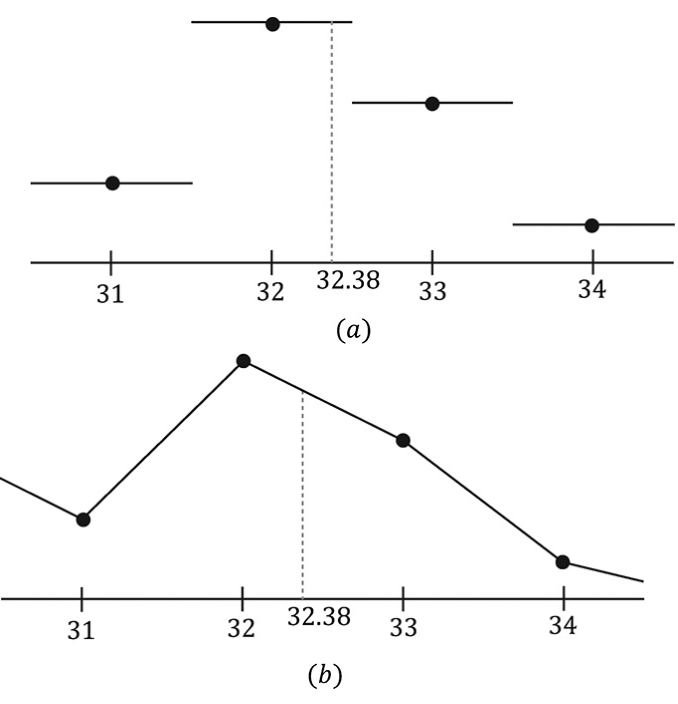
\includegraphics[width=\textwidth]{9-5}
    \centering
    \caption{(a)给定纹素点,我们构造一个分段常数函数来逼近纹素点之间的值; 这有时被称为最近邻点采样,因为使用了最近的纹素点的值。 (b)给定纹素点,我们构造一个分段线性函数来逼近纹素点之间的值。}
\end{figure}

\begin{flushleft}
二维线性插值称为双线性插值,如图\ref{fig:9-6}所示。 给定四个纹素之间的一对纹理坐标,我们在$u$方向上进行两次1D线性插值,然后在$v$方向上进行一次1D插值。
\end{flushleft}

\begin{figure}[h]
    \label{fig:9-6}
    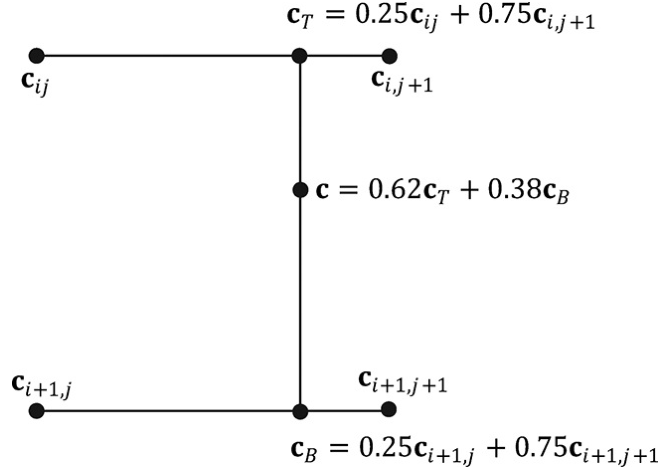
\includegraphics[width=\textwidth]{9-6}
    \centering
    \caption{这里我们有四个纹素点:$c_{ij}$,$c_{i,j+1}$,$c_{i+1,j}$和$c_{i+1,j+1}$。 我们想要使用插值来近似位于这四个纹素点之间的$c$的颜色; 在这个例子中,$c$位于$c_{ij}$右边$0.75$个单位和$c_{ij}$下面$0.38$个单位。 我们首先在前两种颜色之间进行一维线性插值以得到$c_{T}$. 同样,我们在底部两种颜色之间进行一维线性插值以获得$c_{B}$. 最后,我们在$c_{T}$和$c_{B}$之间进行一维线性插值得到$c$。}
\end{figure}

\begin{flushleft}
图\ref{fig:9-7}显示了常量插值和线性插值之间的差异。 如您所见,常量插值具有创建块状图像的特征。 线性插值更平滑,但仍然看起来不真实(例如,更高分辨率的纹理)。\\
\end{flushleft}

\begin{figure}[h]
    \label{fig:9-7}
    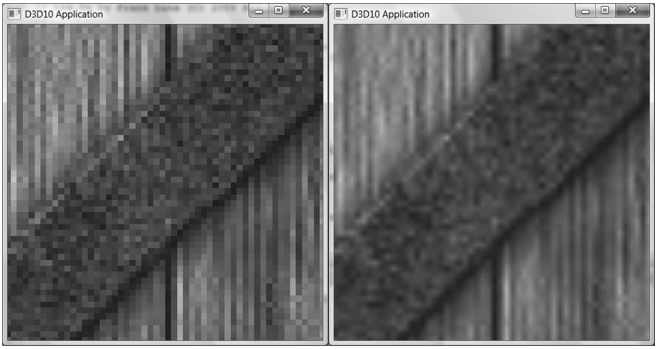
\includegraphics[width=\textwidth]{9-7}
    \centering
    \caption{放大具有板条纹理的立方体。在左边我们使用常数插值,这会出现明显的马赛克; 因为插值函数具有不连续性(图\ref{fig:9-5}a),这使得变化突然而不平滑。 在右侧,我们使用线性过滤,由于插值函数的连续性,出现更平滑的图像效果。}
\end{figure}

%------- 9.5.2 ---------------
\subsection{缩小(Minification)}
\begin{flushleft}
缩小与放大相反。在缩小时,太多的纹素被映射到太少的像素。例如,考虑以下情况,我们在其上绘制了一个$256\times 256$纹理的墙。看着墙壁的眼睛一直向后移动,使墙壁越来越小,直到它只覆盖屏幕上的$64\times 64$像素。所以现在我们有$256\times 256$纹素被映射到$64\times 64$屏幕像素。在这种情况下,像素的纹理坐标通常仍然不与纹理贴图的任何纹素相吻合,因此常量和线性插值滤镜仍然适用于缩小情况。直观地说,应该采用$256\times 256$纹素的一种平均下采样(downsampling)来将其降低到$64\times 64$。mipmapping技术以一些额外的内存为代价提供了有效的近似。在初始化时(或资源创建时),通过对图像进行下采样(downsampling)以创建mipmap链来生成较小版本的纹理(请参见图\ref{fig:9-8})。因此,平均工作是针对mipmap大小预先计算的。在运行时,图形硬件将根据程序员指定的mipmap设置执行两项不同的操作:\\
\end{flushleft}

\begin{itemize}
  \item 1.选择并使用与投影屏幕几何分辨率最匹配的mipmap级别进行纹理处理,根据需要应用常量或线性插值。 这称为mipmap的点过滤(point filtering),因为它类似于常量插值——您只需选择最近的mipmap级别并将其用于纹理。
  \item 2.选择最接近投影屏幕几何分辨率的两个最接近的mipmap级别进行纹理处理(一个将更大,一个将小于屏幕几何分辨率)。 接下来,对这两个mipmap级别应用常量或线性过滤,使每个级别生成纹理颜色。 最后,在这两个纹理颜色结果之间进行插值。 这称为mipmap的线性过滤(linear filtering),因为它类似于线性插值——在两个最近的mipmap级别之间进行线性插值。
\end{itemize}

\begin{flushleft}
通过从mipmap链中选择最佳纹理级别的细节,可以大大减少缩小量。
\end{flushleft}

\begin{figure}[h]
    \label{fig:9-8}
    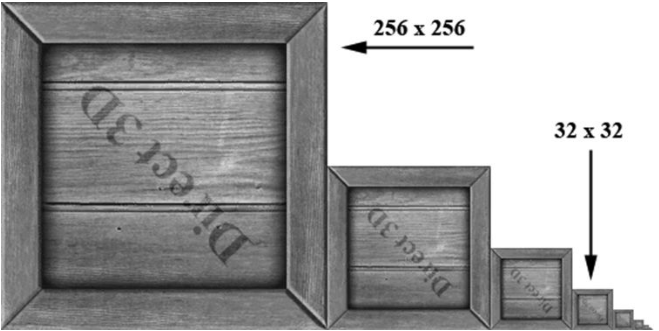
\includegraphics[width=\textwidth]{9-8}
    \centering
    \caption{一个 mipmap 链; 每个连续的mipmap是每个维度的一半大小,前一个mipmap级别的详细信息低至$1\times 1$。}
\end{figure}

\begin{flushleft}
~\\
NOTICE:如9.3.2节所述,可以使用Photoshop DDS导出插件或使用texconv程序创建mipmap。 这些程序使用下采样算法从基本图像数据生成较低的mipmap级别。 有时这些算法不会保留我们想要的细节,艺术家必须手动创建/编辑较低的mipmap级别以保留重要的细节。
~\\
\end{flushleft}

%------- 9.5.3 ---------------
\subsection{各向异性过滤(Anisotropic Filtering)}
\begin{flushleft}
可以使用的另一种类型的过滤器称为各向异性过滤。 该过滤器有助于减轻当多边形的法线向量和相机的外观向量之间的角度较宽时发生的失真(例如,当多边形与视图窗口正交时)。 这种过滤器是最昂贵的,但是可以用于校正失真伪像。 图\ref{fig:9-9}显示了比较各向异性过滤和线性过滤的屏幕截图。
\end{flushleft}

\begin{figure}[h]
    \label{fig:9-9}
    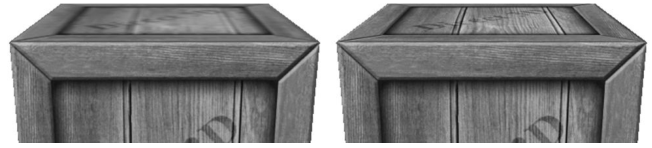
\includegraphics[width=\textwidth]{9-9}
    \centering
    \caption{板条箱的顶面几乎与观察窗口正交。 (左)使用线性过滤条件的顶部非常模糊。 (右)各向异性过滤在从这个角度渲染板条顶面时做得更好。}
\end{figure}

%------- 9.6 ---------------
\section{地址模式(Address Modes)}
\begin{flushleft}
结合常数或线性插值的纹理定义了向量值函数$T(u,v)=(r,g,b,a)$。 也就是说,给定纹理坐标$(u,v)\epsilon [0,1]^{2}$,纹理函数$T$返回颜色$(r,g,b,a)$。 Direct3D允许我们以四种不同的方式(称为地址模式)扩展此功能的域:包裹(wrap),边框颜色(border color),钳位(clamp)和镜像(mirror)。\\
1.包裹(wrap)通过在每个整数结处重复图像来扩展纹理函数(参见图\ref{fig:9-10})。
\end{flushleft}

\begin{figure}[h]
    \label{fig:9-10}
    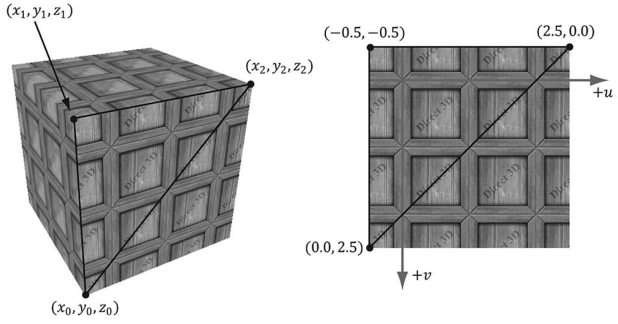
\includegraphics[width=\textwidth]{9-10}
    \centering
    \caption{包裹地址模式。}
\end{figure}

\begin{flushleft}
2.边框颜色(border color)通过将不在$[0,1]^{2}$ 中的每个$(u,v)$映射到程序员指定的某种颜色来扩展纹理功能(参见图\ref{fig:9-11})。
\end{flushleft}

\begin{figure}[h]
    \label{fig:9-11}
    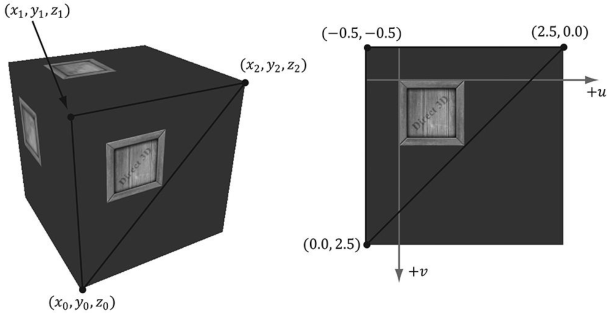
\includegraphics[width=\textwidth]{9-11}
    \centering
    \caption{边框颜色地址模式。}
\end{figure}

\begin{flushleft}
3.钳位(clamp)通过将不在$[0,1]^{2}$中的每个$(u,v)$映射到颜色$T(u_{0},v_{0})$来扩展纹理函数,其中$(u_{0},v_{0})$是最近的点$(u,v)$包含在$[0,1]^{2}$中(见图\ref{fig:9-12})。
\end{flushleft}

\begin{figure}[h]
    \label{fig:9-12}
    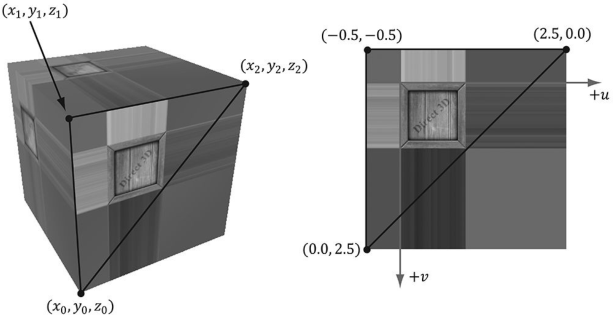
\includegraphics[width=\textwidth]{9-12}
    \centering
    \caption{钳位地址模式。}
\end{figure}

\begin{flushleft}
4.镜像(mirror)通过在每个整数结处镜像图像来扩展纹理函数(参见图\ref{fig:9-13})。
\end{flushleft}

\begin{figure}[h]
    \label{fig:9-13}
    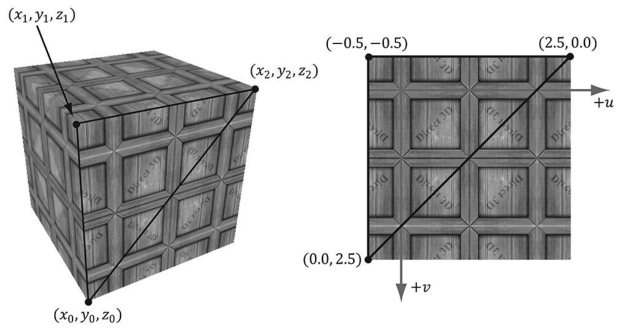
\includegraphics[width=\textwidth]{9-13}
    \centering
    \caption{镜像地址模式。}
\end{figure}

\begin{flushleft}
一个地址模式始终被定义(包裹模式是默认模式),则$[0,1]$范围之外的纹理坐标也被定义。\\
包裹地址模式可能是最常用的; 它允许我们在某些表面上重复平铺纹理。 这有效地使我们能够在不提供额外数据的情况下增加纹理分辨率(尽管额外的分辨率是重复的)。 通过平铺,通常重要的是纹理是无缝的。 例如,板条箱纹理不是无缝的,因为您可以清楚地看到重复。 但是,图\ref{fig:9-14}显示了无缝砖纹理重复$2\times 3$次。
\end{flushleft}

\begin{figure}[h]
    \label{fig:9-14}
    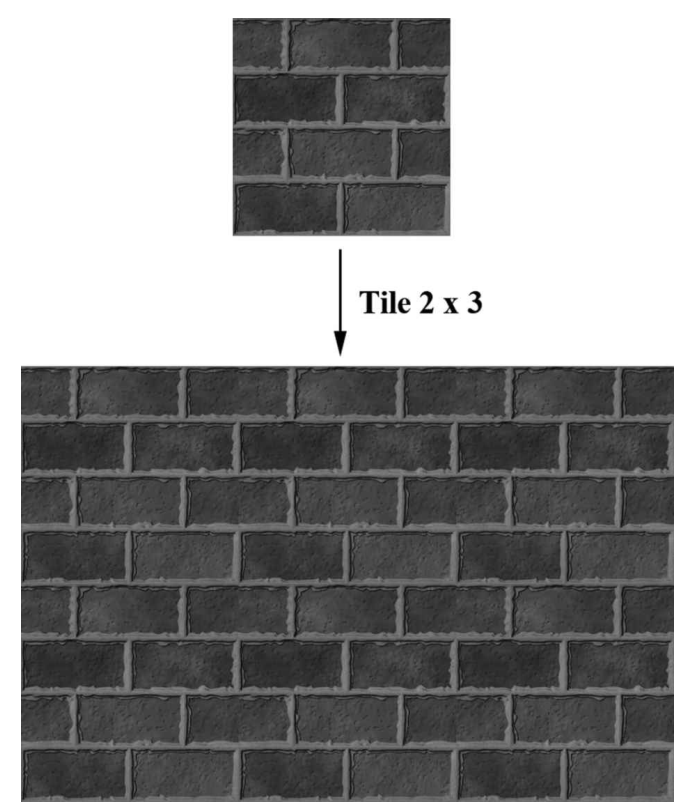
\includegraphics[width=\textwidth]{9-14}
    \centering
    \caption{砖纹理平铺$2\times 3$次。 因为纹理是无缝的,所以重复模式更难以注意到。}
\end{figure}

\clearpage

\begin{flushleft}
地址模式在 Direct3D 中由 D3D12\_TEXTURE\_ADDRESS\_MODE 枚举类定义:\\
\end{flushleft}

\begin{lstlisting}
typedef enum D3D12_TEXTURE_ADDRESS_MODE
{
    D3D12_TEXTURE_ADDRESS_MODE_WRAP = 1,
    D3D12_TEXTURE_ADDRESS_MODE_MIRROR = 2,
    D3D12_TEXTURE_ADDRESS_MODE_CLAMP = 3,
    D3D12_TEXTURE_ADDRESS_MODE_BORDER = 4,
    D3D12_TEXTURE_ADDRESS_MODE_MIRROR_ONCE = 5
} D3D12_TEXTURE_ADDRESS_MODE;
\end{lstlisting}

%------- 9.7 ---------------
\section{采样器对象(Sampler Objects)}
\begin{flushleft}
在前两节中,我们看到除了纹理数据之外,还有两个与使用纹理相关的关键概念:纹理过滤和地址模式。 采样纹理资源时使用的过滤器和地址模式由采样器对象定义。 应用程序通常需要多个采样器对象以不同方式对纹理进行采样。\\
\end{flushleft}

%------- 9.7.1 ---------------
\subsection{创建采样器(Creating Samplers)}
\begin{flushleft}
正如将在下一节中看到的,采样器用于着色器。 为了将采样器绑定到着色器以供使用,我们需要将描述符绑定到采样器对象。 以下代码显示了示例根签名,以便第二个槽采用绑定到采样器寄存器槽0的一个采样器描述符的表。\\
\end{flushleft}

\begin{lstlisting}
CD3DX12_DESCRIPTOR_RANGE descRange[3];
descRange[0].Init(D3D12_DESCRIPTOR_RANGE_TYPE_SRV, 1, 0);
descRange[1].Init(D3D12_DESCRIPTOR_RANGE_TYPE_SAMPLER, 1, 0);
descRange[2].Init(D3D12_DESCRIPTOR_RANGE_TYPE_CBV, 1, 0);
CD3DX12_ROOT_PARAMETER rootParameters[3];
rootParameters[0].InitAsDescriptorTable(
    1,
    &descRange[0], 
    D3D12_SHADER_VISIBILITY_PIXEL);
rootParameters[1].InitAsDescriptorTable(
    1,
    &descRange[1], 
    D3D12_SHADER_VISIBILITY_PIXEL);
rootParameters[2].InitAsDescriptorTable(
    1,
    &descRange[2], 
    D3D12_SHADER_VISIBILITY_ALL);
CD3DX12_ROOT_SIGNATURE_DESC descRootSignature;
descRootSignature.Init(
    3, 
    rootParameters, 
    0, 
    nullptr,
    D3D12_ROOT_SIGNATURE_FLAG_ALLOW_INPUT_ASSEMBLER_INPUT_LAYOUT);
\end{lstlisting}

\begin{flushleft}
如果要设置采样器描述符,需要一个采样器堆。通过填写D3D12\_DESCRIPTOR\_HEAP\_DESC 实例并指定堆类型D3D12\_DESCRIPTOR\_HEAP\_TYPE\_SAMPLER来创建采样器堆:\\
\end{flushleft}

\begin{lstlisting}
D3D12_DESCRIPTOR_HEAP_DESC descHeapSampler = {};
descHeapSampler.NumDescriptors = 1;
descHeapSampler.Type = D3D12_DESCRIPTOR_HEAP_TYPE_SAMPLER;
descHeapSampler.Flags = D3D12_DESCRIPTOR_HEAP_FLAG_SHADER_VISIBLE;
ComPtr<ID3D12DescriptorHeap> mSamplerDescriptorHeap;
ThrowIfFailed(mDevice->CreateDescriptorHeap(
    &descHeapSampler,
    __uuidof(ID3D12DescriptorHeap),
    (void**)&mSamplerDescriptorHeap));
\end{lstlisting}

\begin{flushleft}
一旦有一个采样器堆,就可以创建采样器描述符。 在这里通过填写D3D12\_SAMPLER\_DESC对象来指定地址模式和过滤器类型以及其他参数:\\
\end{flushleft}

\begin{lstlisting}
typedef struct D3D12_SAMPLER_DESC
{
    D3D12_FILTER Filter;
    D3D12_TEXTURE_ADDRESS_MODE AddressU;
    D3D12_TEXTURE_ADDRESS_MODE AddressV;
    D3D12_TEXTURE_ADDRESS_MODE AddressW;
    FLOAT MipLODBias;
    UINT MaxAnisotropy;
    D3D12_COMPARISON_FUNC ComparisonFunc;
    FLOAT BorderColor[4];
    FLOAT MinLOD;
    FLOAT MaxLOD;
} D3D12_SAMPLER_DESC;
\end{lstlisting}

\begin{flushleft}
1. Filter: D3D12\_FILTER枚举类型的成员,用于指定要使用的过滤类型。\\
2. AddressU: 纹理的水平$u$轴方向上的地址模式。\\
3. AddressV: 纹理的垂直$v$轴方向上的地址模式。\\
4. AddressW: 纹理的深度$w$轴方向上的地址模式(仅适用于3D纹理)。\\
5. MipLODBias: 偏移所选择的mipmap级别的值。指定0.0表示无偏差。\\
6. MaxAnisotropy: 最大各向异性值必须在1-16之间。 这仅适用于D3D12\_FILTER\_ANISOTROPIC或D3D12\_FILTER\_COMPARISON\_ANISOTROPIC。较大的值更昂贵,但可以提供更好的结果。\\
7. ComparisonFunc: 高级选项用于某些特定应用程序,如阴影贴图。现在,只需设置为D3D12\_COMPARISON\_FUNC\_ALWAYS,直到影子映射章节。\\
8. BorderColor: 用于指定地址模式 D3D12\_TEXTURE\_ADDRESS\_MODE\_BORDER 的边框颜色。\\
9. MinLOD: 可以选择的最小mipmap级别。\\
10. MaxLOD: 可以选择的最大mipmap级别。\\
~\\
以下是常用 D3D12\_FILTER 类型的一些示例:\\
1. D3D12\_FILTER\_MIN\_MAG\_MIP\_POINT:对纹理贴图进行点过滤,并跨越mipmap级别进行点过滤(即,使用最近的mipmap级别)。\\
2. D3D12\_FILTER\_MIN\_MAG\_LINEAR\_MIP\_POINT:纹理贴图上的双线性滤波,以及跨mipmap级别的点过滤(即,使用最近的mipmap级别)。\\
3. D3D12\_FILTER\_MIN\_MAG\_MIP\_LINEAR:纹理贴图上的双线性滤波,以及两个最近的下部和上部mipmap级别之间的线性滤波。 这通常称为三线性过滤。\\
4. D3D12\_FILTER\_ANISOTROPIC:用于缩小,放大和mipmapping的各向异性过滤。\\
~\\

您可以从这些示例中找出其他可能的排列,或者您可以在SDK文档中查找D3D12\_FILTER枚举类型。\\

以下示例说明如何为堆中的采样器创建描述符,该采样器使用线性过滤,包裹地址模式和其他参数的典型默认值:\\
\end{flushleft}

\begin{lstlisting}
D3D12_SAMPLER_DESC samplerDesc = {};
samplerDesc.Filter = D3D12_FILTER_MIN_MAG_MIP_LINEAR;
samplerDesc.AddressU = D3D12_TEXTURE_ADDRESS_MODE_WRAP;
samplerDesc.AddressV = D3D12_TEXTURE_ADDRESS_MODE_WRAP;
samplerDesc.AddressW = D3D12_TEXTURE_ADDRESS_MODE_WRAP;
samplerDesc.MinLOD = 0;
samplerDesc.MaxLOD = D3D12_FLOAT32_MAX;
samplerDesc.MipLODBias = 0.0f;
samplerDesc.MaxAnisotropy = 1;
samplerDesc.ComparisonFunc = D3D12_COMPARISON_FUNC_ALWAYS;
md3dDevice->CreateSampler(
    &samplerDesc,
    mSamplerDescriptorHeap->GetCPUDescriptorHandleForHeapStart());
\end{lstlisting}

\begin{flushleft}
以下代码显示如何将采样器描述符绑定到根签名参数槽以供着色器程序使用:\\
\end{flushleft}

\begin{lstlisting}
commandList->SetGraphicsRootDescriptorTable(
    1,
    samplerDescriptorHeap->
    GetGPUDescriptorHandleForHeapStart());
\end{lstlisting}

%------- 9.7.2 ---------------
\subsection{静态采样器(Static Samplers)}
\begin{flushleft}
事实证明,图形应用程序通常只使用少数采样器。 因此,Direct3D提供了一个特殊的快捷方式来定义一个采样器数组并设置它们,而无需经过创建采样器堆的过程。 CD3DX12\_ROOT\_SIGNATURE\_DESC 类的Init函数有两个参数,允许您定义应用程序可以使用的所谓静态采样器数组。静态采样器由D3D12\_STATIC\_SAMPLER\_DESC 结构描述。 此结构与D3D12\_SAMPLER\_DESC非常相似,但有以下例外:\\

1.边框颜色可能有一些限制。具体来说,静态采样器的边框颜色必须是以下成员:\\
\end{flushleft}

\begin{lstlisting}
enum D3D12_STATIC_BORDER_COLOR
{
    D3D12_STATIC_BORDER_COLOR_TRANSPARENT_BLACK = 0,
    D3D12_STATIC_BORDER_COLOR_OPAQUE_BLACK = 
        (D3D12_STATIC_BORDER_COLOR_TRANSPARENT_BLACK + 1),
    D3D12_STATIC_BORDER_COLOR_OPAQUE_WHITE = 
        (D3D12_STATIC_BORDER_COLOR_OPAQUE_BLACK + 1)
} D3D12_STATIC_BORDER_COLOR;
\end{lstlisting}

\begin{flushleft}
2. 它包含用于指定着色器寄存器,寄存器空间和着色器的其他字段可见性,通常被指定为采样器堆的一部分。\\

此外,您只能定义2032个静态采样器,这对于大多数应用来说已经足够了。 但是,如果确实需要更多,则可以使用非静态采样器并通过采样器堆。\\
我们在演示中使用静态采样器。 以下代码显示了我们如何定义静态采样器。 请注意,在演示中不需要所有这些静态采样器,但仍然定义它们,以便在需要它们时马上使用。 无论如何,它只是少数,定义一些可能使用或不使用的额外采样器并没有什么坏处。\\
\end{flushleft}

\begin{lstlisting}
std::array<const CD3DX12_STATIC_SAMPLER_DESC, 6> 
TexColumnsApp::GetStaticSamplers()
{
    // Applications usually only need a handful of samplers. 
    // So just define them all up front
    // and keep them available as part of the root signature.  

    const CD3DX12_STATIC_SAMPLER_DESC pointWrap(
        0, // shaderRegister
        D3D12_FILTER_MIN_MAG_MIP_POINT, // filter
        D3D12_TEXTURE_ADDRESS_MODE_WRAP,  // addressU
        D3D12_TEXTURE_ADDRESS_MODE_WRAP,  // addressV
        D3D12_TEXTURE_ADDRESS_MODE_WRAP); // addressW

    const CD3DX12_STATIC_SAMPLER_DESC pointClamp(
        1, // shaderRegister
        D3D12_FILTER_MIN_MAG_MIP_POINT, // filter
        D3D12_TEXTURE_ADDRESS_MODE_CLAMP,  // addressU
        D3D12_TEXTURE_ADDRESS_MODE_CLAMP,  // addressV
        D3D12_TEXTURE_ADDRESS_MODE_CLAMP); // addressW

    const CD3DX12_STATIC_SAMPLER_DESC linearWrap(
        2, // shaderRegister
        D3D12_FILTER_MIN_MAG_MIP_LINEAR, // filter
        D3D12_TEXTURE_ADDRESS_MODE_WRAP,  // addressU
        D3D12_TEXTURE_ADDRESS_MODE_WRAP,  // addressV
        D3D12_TEXTURE_ADDRESS_MODE_WRAP); // addressW

    const CD3DX12_STATIC_SAMPLER_DESC linearClamp(
        3, // shaderRegister
        D3D12_FILTER_MIN_MAG_MIP_LINEAR, // filter
        D3D12_TEXTURE_ADDRESS_MODE_CLAMP,  // addressU
        D3D12_TEXTURE_ADDRESS_MODE_CLAMP,  // addressV
        D3D12_TEXTURE_ADDRESS_MODE_CLAMP); // addressW

    const CD3DX12_STATIC_SAMPLER_DESC anisotropicWrap(
        4, // shaderRegister
        D3D12_FILTER_ANISOTROPIC, // filter
        D3D12_TEXTURE_ADDRESS_MODE_WRAP,  // addressU
        D3D12_TEXTURE_ADDRESS_MODE_WRAP,  // addressV
        D3D12_TEXTURE_ADDRESS_MODE_WRAP,  // addressW
        0.0f,                             // mipLODBias
        8);                               // maxAnisotropy

    const CD3DX12_STATIC_SAMPLER_DESC anisotropicClamp(
        5, // shaderRegister
        D3D12_FILTER_ANISOTROPIC, // filter
        D3D12_TEXTURE_ADDRESS_MODE_CLAMP,  // addressU
        D3D12_TEXTURE_ADDRESS_MODE_CLAMP,  // addressV
        D3D12_TEXTURE_ADDRESS_MODE_CLAMP,  // addressW
        0.0f,                              // mipLODBias
        8);                                // maxAnisotropy

    return { 
        pointWrap, pointClamp,
        linearWrap, linearClamp, 
        anisotropicWrap, anisotropicClamp };
}

void TexColumnsApp::BuildRootSignature()
{
    CD3DX12_DESCRIPTOR_RANGE texTable;
    texTable.Init(
        D3D12_DESCRIPTOR_RANGE_TYPE_SRV, 
        1,  // number of descriptors
        0); // register t0

    // Root parameter can be a table, root descriptor 
    // or root constants.
    CD3DX12_ROOT_PARAMETER slotRootParameter[4];

    // Perfomance TIP: Order from most frequent 
    // to least frequent.
    slotRootParameter[0].InitAsDescriptorTable(
        1, 
        &texTable, 
        D3D12_SHADER_VISIBILITY_PIXEL);
    // register b0
    slotRootParameter[1].InitAsConstantBufferView(0);
    // register b1
    slotRootParameter[2].InitAsConstantBufferView(1);
    // register b2
    slotRootParameter[3].InitAsConstantBufferView(2);

    auto staticSamplers = GetStaticSamplers();

    // A root signature is an array of root parameters.
    CD3DX12_ROOT_SIGNATURE_DESC rootSigDesc(
        4, 
        slotRootParameter,
        (UINT)staticSamplers.size(), 
        staticSamplers.data(),
        D3D12_ROOT_SIGNATURE_FLAG_ALLOW_INPUT_ASSEMBLER_INPUT_LAYOUT);

    // create a root signature with a single slot 
    // which points to a descriptor range consisting 
    // of a single constant buffer
    ComPtr<ID3DBlob> serializedRootSig = nullptr;
    ComPtr<ID3DBlob> errorBlob = nullptr;
    HRESULT hr = D3D12SerializeRootSignature(
        &rootSigDesc, D3D_ROOT_SIGNATURE_VERSION_1,
        serializedRootSig.GetAddressOf(), 
        errorBlob.GetAddressOf());

    if(errorBlob != nullptr)
    {
        ::OutputDebugStringA((char*)errorBlob->
        GetBufferPointer());
    }
    ThrowIfFailed(hr);

    ThrowIfFailed(md3dDevice->CreateRootSignature(
        0,
        serializedRootSig->GetBufferPointer(),
        serializedRootSig->GetBufferSize(),
        IID_PPV_ARGS(mRootSignature.GetAddressOf())));
}
\end{lstlisting}

%------- 9.8 ---------------
\section{在着色器中采样纹理(Sampling Textures In A Shader)}
\begin{flushleft}
纹理对象在HLSL中定义,并使用以下语法分配给纹理寄存器:\\
\end{flushleft}

\begin{lstlisting}
Texture2D gDiffuseMap : register(t0);
\end{lstlisting}

\begin{flushleft}
请注意,纹理寄存器使用由$tn$指定,其中$n$是标识纹理寄存器槽的整数。 根签名定义指定从slot参数到着色器寄存器的映射; 这是应用程序代码如何将SRV绑定到着色器中的特定Texture2D对象。\\

类似地,采样器对象定义为HLSL,并使用以下语法分配给采样器寄存器:\\
\end{flushleft}

\begin{lstlisting}
SamplerState gsamPointWrap : register(s0);
SamplerState gsamPointClamp : register(s1);
SamplerState gsamLinearWrap : register(s2);
SamplerState gsamLinearClamp : register(s3);
SamplerState gsamAnisotropicWrap : register(s4);
SamplerState gsamAnisotropicClamp : register(s5);
\end{lstlisting}

\begin{flushleft}
这些采样器对应于我们在上一节中设置的静态采样器阵列。 请注意,纹理寄存器使用$sn$指定,其中$n$是标识采样器寄存器槽的整数。\\
现在,给定像素着色器中像素的一对纹理坐标$(u,v)$,我们实际使用 Texture2D::Sample 方法对纹理进行采样:\\
\end{flushleft}

\begin{lstlisting}
Texture2D gDiffuseMap : register(t0);
SamplerState gsamPointWrap : register(s0);
SamplerState gsamPointClamp : register(s1);
SamplerState gsamLinearWrap : register(s2);
SamplerState gsamLinearClamp : register(s3);
SamplerState gsamAnisotropicWrap : register(s4);
SamplerState gsamAnisotropicClamp : register(s5);

struct VertexOut
{
    float4 PosH : SV_POSITION;
    float3 PosW : POSITION;
    float3 NormalW : NORMAL;
    float2 TexC : TEXCOORD;
};

float4 PS(VertexOut pin) : SV_Target
{
    float4 diffuseAlbedo =
    gDiffuseMap.Sample(gsamAnisotropicWrap, pin.TexC) *
    gDiffuseAlbedo;
    ...
\end{lstlisting}

\begin{flushleft}
我们为第一个参数传递一个SamplerState对象,表示如何对纹理数据进行采样,并为第二个参数传递像素的$(u,v)$纹理坐标。 此方法使用 SamplerState 对象指定的过滤方法从指定$(u,v)$点处的纹理贴图返回插值颜色。\\
\end{flushleft}


%------- 9.9 ---------------
\section{条箱演示(Crate Demo)}
\begin{flushleft}
现在回顾一下将条箱(crate)纹理添加到多维数据集的关键点(如图\ref{fig:9-1}所示)。
\end{flushleft}

%------- 9.9.1 ---------------
\subsection{设定纹理坐标(Specifying Texture Coordinates)}
\begin{flushleft}
GeometryGenerator::CreateBox 生成箱(box)的纹理坐标,以便将整个纹理图像映射到箱的每个面上。 为简洁起见,我们仅显示正面,背面和顶面的顶点定义。 另请注意,我们省略了顶点构造函数中法线和切线向量的坐标(纹理坐标以粗体显示)。\\
\end{flushleft}

\begin{lstlisting}[escapechar=^]
GeometryGenerator::MeshData
GeometryGenerator::CreateBox(
float width, float height, float depth,
uint32 numSubdivisions)
{
    MeshData meshData;
    Vertex v[24];
    float w2 = 0.5f*width;
    float h2 = 0.5f*height;
    float d2 = 0.5f*depth;
    // Fill in the front face vertex data.
    v[0] = Vertex(..., ^\textbf{1.0f, 0.0f, 0.0f}^, ...);
    v[1] = Vertex(..., ^\textbf{1.0f, 0.0f, 0.0f}^, ...);
    v[2] = Vertex(..., ^\textbf{1.0f, 0.0f, 0.0f}^, ...);
    v[3] = Vertex(..., ^\textbf{1.0f, 0.0f, 0.0f}^, ...);
    // Fill in the back face vertex data.
    v[4] = Vertex(..., ^\textbf{-1.0f, 0.0f, 0.0f}^, ...);
    v[5] = Vertex(..., ^\textbf{-1.0f, 0.0f, 0.0f}^, ...);
    v[6] = Vertex(..., ^\textbf{-1.0f, 0.0f, 0.0f}^, ...);
    v[7] = Vertex(..., ^\textbf{-1.0f, 0.0f, 0.0f}^, ...);
     // Fill in the top face vertex data.
    v[8] = Vertex(..., ^\textbf{1.0f, 0.0f, 0.0f}^, ...);
    v[9] = Vertex(..., ^\textbf{1.0f, 0.0f, 0.0f}^, ...);
    v[10] = Vertex(..., ^\textbf{1.0f, 0.0f, 0.0f}^, ...);
    v[11] = Vertex(..., ^\textbf{1.0f, 0.0f, 0.0f}^, ...);
\end{lstlisting}

\begin{flushleft}
如果需要帮助,请查看为什么以这种方式指定纹理坐标,请参见图\ref{fig:9-3}。
\end{flushleft}

%------- 9.9.2 ---------------
\subsection{创建纹理(Creating the Texture)}
\begin{flushleft}
在初始化通过文件创建纹理,如下所示:\\
\end{flushleft}

\begin{lstlisting}
// Helper structure to group data related to the texture.
struct Texture
{
    // Unique material name for lookup.
    std::string Name;
    std::wstring Filename;
    Microsoft::WRL::ComPtr<ID3D12Resource> Resource =
        nullptr;
    Microsoft::WRL::ComPtr<ID3D12Resource> UploadHeap =
        nullptr;
};

std::unordered_map<std::string,
    std::unique_ptr<Texture>> mTextures;
void CrateApp::LoadTextures()
{
    auto woodCrateTex = std::make_unique<Texture>();
    woodCrateTex->Name = “woodCrateTex”;
    woodCrateTex->Filename = L”Textures/WoodCrate01.dds”;
    ThrowIfFailed(DirectX::CreateDDSTextureFromFile12(
        md3dDevice.Get(),
        mCommandList.Get(), 
        woodCrateTex->Filename.c_str(),
        woodCrateTex->Resource, 
        woodCrateTex->UploadHeap));
    mTextures[woodCrateTex->Name] =
        std::move(woodCrateTex);
}
\end{lstlisting}

\begin{flushleft}
将所有独特纹理存储在unordered map中,以便我们可以按名称查找它们。 在生产代码中,在加载纹理之前,您需要检查纹理数据是否已经加载(即,它是否已经包含在unordered map中),以便它不会多次加载。\\
\end{flushleft}

%------- 9.9.3 ---------------
\subsection{设置纹理(Setting the Texture)}
\begin{flushleft}
一旦创建了纹理并在描述符堆中为它创建了SRV,将纹理绑定到管道就可以在着色器程序中使用。接下来只需将其设置为需要纹理的根签名参数:\\
\end{flushleft}

\begin{lstlisting}
// Get SRV to texture we want to bind.
CD3DX12_GPU_DESCRIPTOR_HANDLE tex(
    mSrvDescriptorHeap->
    GetGPUDescriptorHandleForHeapStart());
tex.Offset(
    ri->Mat->DiffuseSrvHeapIndex,
    mCbvSrvDescriptorSize);
...
// Bind to root parameter 0. The root parameter
// description specifies which
// shader register slot this corresponds to.
cmdList->SetGraphicsRootDescriptorTable(0, tex);
\end{lstlisting}

%------- 9.9.4 ---------------
\subsection{更新 HLSL(Updated HLSL)}
\begin{flushleft}
下面是修改后的 Default.hlsl 文件,现在支持纹理(纹理代码已加粗):\\
\end{flushleft}

\begin{lstlisting}[escapechar=^]
//*********************************************************
// Default.hlsl by Frank Luna (C) 2015 All Rights Reserved.
//*********************************************************

// Defaults for number of lights.
#ifndef NUM_DIR_LIGHTS
    #define NUM_DIR_LIGHTS 3
#endif

#ifndef NUM_POINT_LIGHTS
    #define NUM_POINT_LIGHTS 0
#endif

#ifndef NUM_SPOT_LIGHTS
    #define NUM_SPOT_LIGHTS 0
#endif

// Include structures and functions for lighting.
#include "LightingUtil.hlsl"

Texture2D    gDiffuseMap : register(t0);


SamplerState gsamPointWrap        : register(s0);
SamplerState gsamPointClamp       : register(s1);
SamplerState gsamLinearWrap       : register(s2);
SamplerState gsamLinearClamp      : register(s3);
SamplerState gsamAnisotropicWrap  : register(s4);
SamplerState gsamAnisotropicClamp : register(s5);

// Constant data that varies per frame.
cbuffer cbPerObject : register(b0)
{
    float4x4 gWorld;
    ^\textbf{float4x4 gTexTransform;}^
};

// Constant data that varies per material.
cbuffer cbPass : register(b1)
{
    float4x4 gView;
    float4x4 gInvView;
    float4x4 gProj;
    float4x4 gInvProj;
    float4x4 gViewProj;
    float4x4 gInvViewProj;
    float3 gEyePosW;
    float cbPerObjectPad1;
    float2 gRenderTargetSize;
    float2 gInvRenderTargetSize;
    float gNearZ;
    float gFarZ;
    float gTotalTime;
    float gDeltaTime;
    float4 gAmbientLight;

    // Indices [0, NUM_DIR_LIGHTS) are directional lights;
    // indices [NUM_DIR_LIGHTS, NUM_DIR_LIGHTS+NUM_POINT_LIGHTS) are point lights;
    // indices [NUM_DIR_LIGHTS+NUM_POINT_LIGHTS, NUM_DIR_LIGHTS+NUM_POINT_LIGHT+NUM_SPOT_LIGHTS)
    // are spot lights for a maximum of MaxLights per object.
    Light gLights[MaxLights];
};

cbuffer cbMaterial : register(b2)
{
    float4   gDiffuseAlbedo;
    float3   gFresnelR0;
    float    gRoughness;
    ^\textbf{float4x4 gMatTransform;}^
};

struct VertexIn
{
    float3 PosL    : POSITION;
    float3 NormalL : NORMAL;
    ^\textbf{float2 TexC    : TEXCOORD;}^
};

struct VertexOut
{
    float4 PosH    : SV_POSITION;
    float3 PosW    : POSITION;
    float3 NormalW : NORMAL;
    ^\textbf{float2 TexC    : TEXCOORD;}^
};

VertexOut VS(VertexIn vin)
{
    VertexOut vout = (VertexOut)0.0f;
    
    // Transform to world space.
    float4 posW = mul(float4(vin.PosL, 1.0f), gWorld);
    vout.PosW = posW.xyz;

    // Assumes nonuniform scaling; otherwise, need to use 
    // inverse-transpose of world matrix.
    vout.NormalW = mul(vin.NormalL, (float3x3)gWorld);

    // Transform to homogeneous clip space.
    vout.PosH = mul(posW, gViewProj);
    
    ^\textbf{// Output vertex attributes for }^
    ^\textbf{// interpolation across triangle.}^
    ^\textbf{float4 texC = mul(float4(vin.TexC, 0.0f, 1.0f), gTexTransform);}^
    ^\textbf{vout.TexC = mul(texC, gMatTransform).xy;}^
    
    return vout;
}

float4 PS(VertexOut pin) : SV_Target
{
    ^\textbf{float4 diffuseAlbedo = }^
       ^\textbf{gDiffuseMap.Sample(gsamAnisotropicWrap, pin.TexC) *}^
       ^\textbf{gDiffuseAlbedo;}^
    
    // Interpolating normal can unnormalize it, so renormalize it.
    pin.NormalW = normalize(pin.NormalW);

    // Vector from point being lit to eye. 
    float3 toEyeW = normalize(gEyePosW - pin.PosW);

    // Light terms.
    float4 ambient = gAmbientLight*diffuseAlbedo;

    const float shininess = 1.0f - gRoughness;
    Material mat = { diffuseAlbedo, gFresnelR0, shininess };
    float3 shadowFactor = 1.0f;
    float4 directLight = ComputeLighting(gLights, mat, pin.PosW,
        pin.NormalW, toEyeW, shadowFactor);

    float4 litColor = ambient + directLight;

    // Common convention to take alpha from diffuse albedo.
    litColor.a = diffuseAlbedo.a;

    return litColor;
}
\end{{lstlisting}

%------- 9.10 ---------------
\section{纹理转换(Transforming Textures)}
\begin{flushleft}
我们没有讨论过的两个常量缓冲区变量是gTexTransform和gMatTransform。 这些变量在顶点着色器中用于变换输入纹理坐标:\\
\end{flushleft}

\begin{lstlisting}
// Output vertex attributes for 
// interpolation across triangle.
float4 texC = mul(float4(vin.TexC, 0.0f, 1.0f),
                  gTexTransform);
vout.TexC = mul(texC, gMatTransform).xy;
\end{lstlisting}

\begin{flushleft}
纹理坐标表示纹理平面中的2D点。因此,可以像任何其他点一样平移、旋转和缩放它们。 以下是转换纹理的一些示例用法:\\
1.砖纹理沿墙壁被拉伸。墙顶点当前具有范围$[0,1]$中的纹理坐标。将纹理坐标缩放$4$倍,则范围变为$[0,4]$,这样纹理将在墙上重复4乘4(four-by-four)次。\\

2.云纹理在清澈的蓝天延伸。通过将纹理坐标转换为时间的函数,云在天空上呈现动画效果。\\

3.纹理旋转有时对粒子效果非常有用,例如,我们会随着时间的推移旋转火球纹理。\\

在“条箱”演示中,使用单位矩阵变换,以便输入纹理坐标保持不变,在下一节中,将解释使用纹理变换的演示。\\
请注意,要将2D纹理坐标转换为$4\times 4$矩阵,我们将其扩展为4D向量:\\
\end{flushleft}

\begin{lstlisting}
vin.TexC -> float4(vin.Tex, 0,0f, 1.0f)
\end{lstlisting}

\begin{flushleft}
在乘法完成之后,通过丢弃$z$分量和$w$分量将得到的4D向量回送到2D向量。 那是,\\
\end{flushleft}

\begin{lstlisting}
vout.TexC = mul(float4(vin.TexC, 0.0f, 1.0f), gTexTransform).xy;
\end{lstlisting}

\begin{flushleft}
使用两个单独的纹理变换矩阵 gTexTransform 和 gMatTransform,因为有时这种做法对材质转换纹理(对于像水这样的动画材料)很有帮助,但有时它使纹理变换成为对象的属性更方便。\\

因为正在处理2D纹理坐标,所以我们只关心对前两个坐标进行的转换。 例如,如果纹理矩阵转换了$z$坐标,则它对结果纹理坐标没有影响。\\
\end{flushleft}

%------- 9.11 ---------------
\section{纹理的小山和波浪演示(Textured Hills And Waves Demo)}
\begin{flushleft}
在这个演示中,为陆地和水场景添加纹理。第一个关键问题是在土地上铺设草纹。 因为陆地网格是一个大的表面,如果我们简单地在其上拉伸纹理,那么太少的纹素将覆盖每个三角形。 换句话说,表面没有足够的纹理分辨率; 因此我们会得到放大的效果。 因此,需要在陆地网格上重复草纹理以获得更高的分辨率。 第二个关键问题是在水几何上随时间函数滚动水纹理。这种简单动画使水更有说服力。 图\ref{fig:9-15}显示了演示的屏幕截图。\\
\end{flushleft}

\begin{figure}[h]
    \label{fig:9-15}
    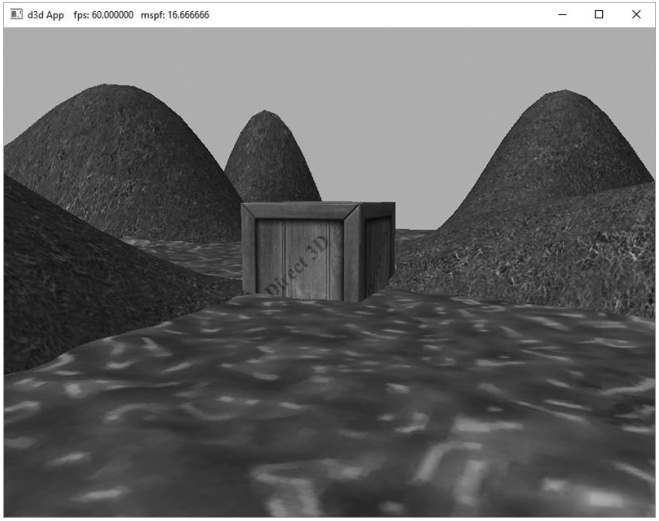
\includegraphics[width=\textwidth]{9-15}
    \centering
    \caption{地面纹理演示截图}
\end{figure}

%------- 9.11.1 ---------------
\subsection{网格纹理坐标生成(Grid Texture Coordinate Generation)}
\begin{flushleft}
图\ref{fig:9-16}显示了$xz$平面中的$m\times n$网格和归一化纹理空间域$[0,1]^{2}$中的对应网格。 从图中可以清楚地看出,$xz$平面中第$i$个网格顶点的纹理坐标是纹理空间中第$i$个网格顶点的坐标。 第$i$个顶点的纹理空间坐标是:\\
\end{flushleft}

\begin{align*}
u_{ij}&=j\cdot \Delta u\\
v_{ij}&=i\cdot \Delta v
where \Delta u=\frac{1}{n-1} and \Delta v=\frac{1}{m-1}
\end{align*}

\begin{figure}[h]
    \label{fig:9-16}
    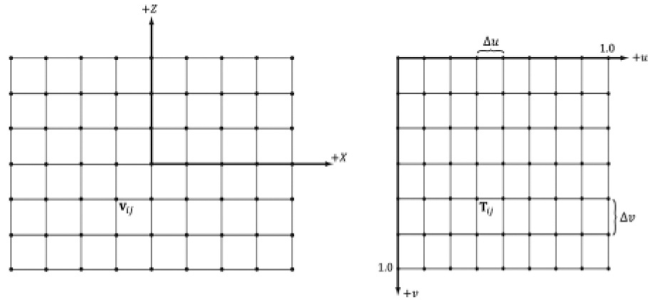
\includegraphics[width=\textwidth]{9-16}
    \centering
    \caption{$xz$空间中的网格顶点$v_{ij}$的纹理坐标由$uv$空间中的第$i$个网格顶点$T_{ij}$给出。}
\end{figure}

\begin{flushleft}
因此,使用以下代码在 GeometryGenerator::CreateGrid 方法中为网格生成纹理坐标:\\
\end{flushleft}

\begin{lstlisting}[escapechar=^]
GeometryGenerator::MeshData 
GeometryGenerator::CreateGrid(
    float width,
    float depth,
    uint32 m,
    uint32 n)
{
    MeshData meshData;

    uint32 vertexCount = m*n;
    uint32 faceCount   = (m-1)*(n-1)*2;

    //
    // Create the vertices.
    //

    float halfWidth = 0.5f*width;
    float halfDepth = 0.5f*depth;

    float dx = width / (n-1);
    float dz = depth / (m-1);

    ^\textbf{float du = 1.0f / (n-1);}^
    ^\textbf{float dv = 1.0f / (m-1);}^

    meshData.Vertices.resize(vertexCount);
    for(uint32 i = 0; i < m; ++i)
    {
        float z = halfDepth - i*dz;
        for(uint32 j = 0; j < n; ++j)
        {
            float x = -halfWidth + j*dx;

            meshData.Vertices[i*n+j].Position = XMFLOAT3(x, 0.0f, z);
            meshData.Vertices[i*n+j].Normal   = XMFLOAT3(0.0f, 1.0f, 0.0f);
            meshData.Vertices[i*n+j].TangentU = XMFLOAT3(1.0f, 0.0f, 0.0f);

            ^\textbf{// Stretch texture over grid.}^
            ^\textbf{meshData.Vertices[i*n+j].TexC.x = j*du;}^
            ^\textbf{meshData.Vertices[i*n+j].TexC.y = i*dv;}^
        }
    }
    ...
}
\end{lstlisting}

%------- 9.11.2 ---------------
\subsection{纹理平铺(Texture Tiling)}
\begin{flushleft}
我们说在土地网格上铺设草纹。但到目前为止,计算的纹理坐标位于单位域$[0,1]^{2}$; 所以不会发生平铺。 要平铺纹理,指定包裹地址模式,并使用纹理变换矩阵将纹理坐标缩放到5倍。 这样一来,纹理坐标被映射到域$[0,5]^{2}$,以便纹理在平面网格表面上平铺$5\times 5$次:\\
\end{flushleft}
\begin{lstlisting}
void TexWavesApp::BuildRenderItems()
{
    auto gridRitem = std::make_unique<RenderItem>();
    gridRitem->World = MathHelper::Identity4x4();
    XMStoreFloat4x4(&gridRitem->TexTransform,
    XMMatrixScaling(5.0f, 5.0f, 1.0f));
    ...
}
\end{lstlisting}

%------- 9.11.3 ---------------
\subsection{纹理动画(Texture Animation)}
\begin{flushleft}
要在水几何体上滚动水纹理,将纹理平面中的纹理坐标转换为AnimateMaterials方法中的时间函数,该方法在每个更新周期调用。 如果每帧的位移很小,则会产生平滑动画的错觉。 使用包裹地址模式和无缝纹理,以便我们可以无缝地转换纹理空间平面周围的纹理坐标。 以下代码显示了如何计算水纹理的偏移向量,以及如何构建和设置水的纹理矩阵:\\
\end{flushleft}

\begin{lstlisting}
void TexWavesApp::AnimateMaterials(const GameTimer& gt)
{
    // Scroll the water material texture coordinates.
    auto waterMat = mMaterials["water"].get();

    float& tu = waterMat->MatTransform(3, 0);
    float& tv = waterMat->MatTransform(3, 1);

    tu += 0.1f * gt.DeltaTime();
    tv += 0.02f * gt.DeltaTime();

    if(tu >= 1.0f)
        tu -= 1.0f;

    if(tv >= 1.0f)
        tv -= 1.0f;

    waterMat->MatTransform(3, 0) = tu;
    waterMat->MatTransform(3, 1) = tv;

    // Material has changed, so need to update cbuffer.
    waterMat->NumFramesDirty = gNumFrameResources;
}
\end{lstlisting}

%------- 9.12---------------
\section{总结}
\begin{flushleft}
1.纹理坐标用于定义纹理上的三角形,该三角形映射到3D三角形。\\
2.为游戏创建纹理的最流行的方法是让艺术家在Photoshop或其他图像编辑器中制作它们,然后将它们保存为图像文件,如BMP,DDS,TGA或PNG。 然后游戏应用程序将加载时的图像数据加载到ID3D12Resource对象中。 对于实时图形应用程序,DDS(DirectDraw表面格式)图像文件格式是首选,因为它支持GPU本身理解的各种图像格式; 特别是,它支持可由GPU本机解压缩的压缩图像格式。\\
3.将传统图像格式转换为DDS格式有两种常用方法:使用导出到DDS的图像编辑器或使用名为texconv的Microsoft命令行工具。\\
4.我们可以使用 CreateDDSTextureFromFile12 函数从存储在磁盘上的图像文件创建纹理,该函数位于DVD上的Common/DDSTextureLoader.h/.cpp。\\
5.当我们放大表面并试图用几个纹素覆盖太多屏幕像素时,会发生放大(有马赛克)。 当我们缩小表面并且太多纹素正试图覆盖太少的屏幕像素时,会发生缩小(不平滑)。 Mipmap和纹理过滤器是处理放大和缩小的技术。 GPU本身支持三种纹理过滤(按质量最低,质量较低,质量最高,最昂贵):点,线性和各向异性过滤器。\\
6.地址模式定义了Direct3D应该对$[0,1]$范围之外的纹理坐标做什么。 例如,纹理应该是平铺,镜像,钳位等吗?\\
7.纹理坐标可以像其他点一样缩放,旋转和平移。 通过每帧少量地逐渐变换纹理坐标,可以将纹理设置动画。
\end{flushleft}

%------- 9.13---------------
\section{练习}
\begin{flushleft}
1.通过更改纹理坐标并使用不同的地址模式组合和过滤选项来试验“条箱”演示。 特别是,再现图\ref{fig:9-7},\ref{fig:9-9},\ref{fig:9-10},\ref{fig:9-11},\ref{fig:9-12}和\ref{fig:9-13}中的图像。\\
2.使用DirectX纹理工具,我们可以手动指定每个mipmap级别(File->Open Onto This Surface)。 创建一个带有mipmap链的DDS文件,如图\ref{fig:9-17}所示,在每个级别上使用不同的文本描述或颜色,以便您可以轻松区分每个mipmap级别。 使用此纹理修改条箱演示并让相机放大和缩小,以便您可以明确地看到mipmap级别发生变化。 尝试点和线性mipmap过滤。\\
\end{flushleft}
\begin{figure}[h]
    \label{fig:9-17}
    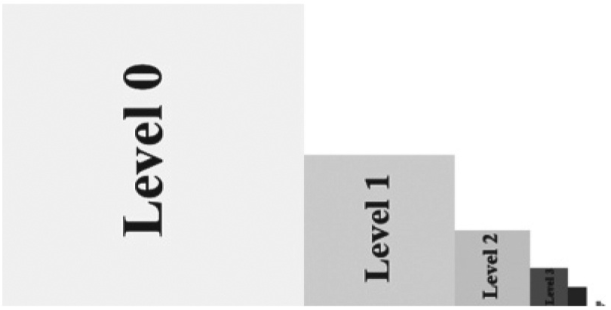
\includegraphics[width=\textwidth]{9-17}
    \centering
    \caption{手动构建的mipmap链,以便每个级别都可以轻松区分。}
\end{figure}

\begin{flushleft}
3.给定两个相同大小的纹理,我们可以通过不同的操作将它们组合起来以获得新的图像。 更一般地,这被称为多纹理,其中使用多个纹理来实现结果。 例如,我们可以添加,减去或(分量)乘以两个纹理的相应纹素。 图\ref{fig:9-18}显示了分量乘以两个纹理以获得类似火球的结果。 在本练习中,通过在图像着色器中组合图\ref{fig:9-18}中的两个源纹理来修改“条箱”演示,使在每个立方体面上生成火球纹理。 (本练习的图像文件可以从本书的网站下载。)请注意,您必须修改Default.hlsl以支持多个纹理。
\end{flushleft}
\begin{figure}[h]
    \label{fig:9-18}
    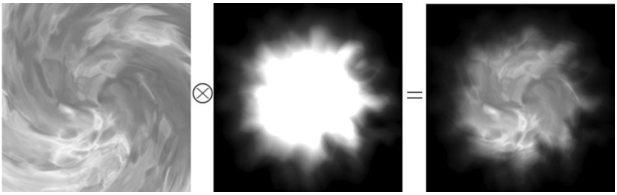
\includegraphics[width=\textwidth]{9-18}
    \centering
    \caption{手动构建的mipmap链,以便每个级别都可以轻松区分。}
\end{figure}

\begin{flushleft}
4.通过在每个立方体面上旋转火球纹理作为时间的函数,将解决方案修改为练习3。\\

5.令$p_{0}$,$p_{1}$和$p_{2}$为具有相应纹理坐标$q_{0}$,$q_{1}$和$q_{2}$的3D三角形的顶点。回想9.2节对于三角形上的任意点$p(s,t)=p_{0}+s(p_{1}-p_{0})+t(p_{2}-p_{0})$其中$s\geq 0$,$t\geq 0$,$s+t\leq 1$,其纹理坐标$(u,v)$是通过相同的$s$,$t$参数在3D三角形上线性插值顶点纹理坐标而得到的:\\
\end{flushleft}
\begin{align*}
(u,v)=q_{0}+s(q_{1}-q_{0})+t(q_{2}-q_{0})
\end{align*}

\begin{itemize}
  \item a.给定$(u,v)$和$q_{0}$,$q_{1}$和$q_{2}$,用$u$和$v$求解$(s,t)$(提示:考虑向量方程$(u,v)=q_{0}+s(q_{1}-q_{0})+t(q_{2}-q_{0})$。
  \item b.表达$p$作为$u$和$v$的函数; 也就是说,找到一个公式$p=p(u,v)$。
  \item c.计算$\partial p/\partial u$和$\partial p/\partial v$并给出这些向量的含义的几何解释。
\end{itemize}

\begin{flushleft}
6.通过向地面,列和球体添加纹理来修改上一章中的“LitColumns”演示(图\ref{9-19})。 纹理可以在本章的代码目录中找到。
\end{flushleft}

\begin{figure}[h]
    \label{fig:9-19}
    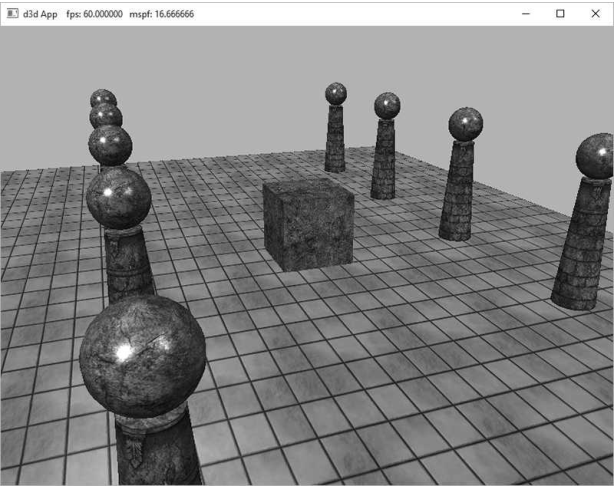
\includegraphics[width=\textwidth]{9-19}
    \centering
    \caption{纹理列场景}
\end{figure}





